\Chapter{SQL lekérdezések végrehajtása}

\Section{Execution Plan}

A lekérdezés végrehajtási terv elkészítésével információkat nyerhetünk a lekérdezések hatékonyságáról. Ennek segítségével optimalizálhatjuk például egy olyan weboldal működését, mely sok és bonyolultabb lekérdezést végez adatbázisból. A hatékonyságot általában indexek hozzáadásával vagy elvételével illetve a táblák kapcsolási sorrendjének módosításával vagy kocsolási módjának megváltoztatásával segíthetjük elő.

\Section{Az \texttt{EXPLAIN} parancs}

A MySQL adatbázismotorban az Executing Plan -hez szükséges információkat az EXPLAIN parancsal használatával kaphatjuk meg.
A parancs megfelelő utasítással együtt használva (SELECT, DELETE, INSERT, REPLACE, UPDATE)  információkat jelenít meg az optimalizáló által előállított feldolgozási tervről. Láthatóvá válik például a táblák összekapcsolási sorrendje.

További információk érhetők el a SHOW WARNINGS használatával.
A FORMAT parancs használható kimeneti formátum választásra. TRADITIONAL az alapértelmezett táblázatos alak. JSON pedig JSON formátumban jeleníti meg a kimenetet.

A parancs használata rávilágít arra, hol van szükség indexek használatára a lekérdezés gyorsításához, illetve ellenőrizhetjük, hogy a táblák megfelelő sorrendben vannak -e összekapcsolva. 
JOIN helyett STRAIGHT\_JOIN használatával tippek adhatóak az optimalizálónak, a táblák kapcsolási sorrendjéről. De a STRAIGHT\_JOIN letiltja a semijoin transzformációkat, így indexelés ebben az esetben nem használható.
ANALYZE TABLE paranccsal frissíthetőek a statisztikák, mint a kulcsok számossága. Ez befolyásolhatja az optimalizáló döntéseit. 

% TODO: Ide érdemes kifejteni, MySQL Workbench-es példákkal illusztrálni, hogy hogyan működik a parancs.

\Section{Teszt adatbázis megtervezése}

Az execution plan optimalizálási módnál a kapott információk felhasználásával tudjuk optimalizálni a lekérdezéseket.
Olyan adatbázist kell választanunk ennek kipróbáláshoz amelyben használhatók indexek de nincs feltétlen szükség rájuk, össze kapcsolhatunk több táblát és rendezhetjük az adatokat például növekvő sorrendben. A felhasználási mód miatt kevés dologra kell ügyelnünk a tábláknál, ilyen például a NotNull. A táblák minden eleme INT típusú, és csak a feltöltött adatok értékének intervalluma tér el. Az elsődleges kulcs minden esetben 0 -tól N-1 ig tart.

\begin{figure}[h!]
\centering
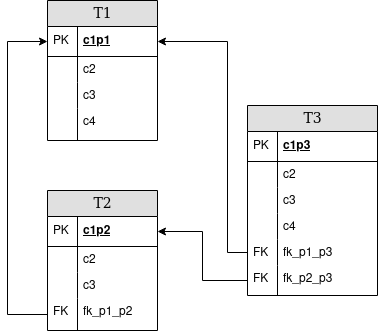
\includegraphics[width=\textwidth]{images/new_schema.png}
\caption{Adatbázis séma}
\label{fig:schema}
\end{figure}

T1 -es tábla:
\begin{itemize}
\item 100 elemet tartalmaz.
\item c2    random érték [1:2] intervallumon.
\item c3    [1:100]
\item c4    [1:10000]
\end{itemize}
T2 -es tábla:
\begin{itemize}
\item 1000 elemet tartalmaz.
\item c2    [1:100]
\item c3    [1:10000]
\end{itemize}
Létrehozás során ügyeltem arra, hogy minden T1.c1p1 kulcshoz tartozzon legalább egy idegen kulcs ebben a táblában.

T3 -as tábla:
\begin{itemize}   
\item 50.000 elemet tartalmaz
\item c2    [1:100]
\item c3    [1:10000]
\item c4    [1:10]
\end{itemize}
Az idegen kulcsok véletlenszerűen kapcsolódnak a T1 -es és T2 -es táblához.


%Az oszlopnevek számozottak. A \texttt{c3}-\texttt{c5} Az értékeik véletlenszerűen generált egészek, \texttt{c3} $in [0, 100]$, \texttt{c4} $in [0, 10000]$, \texttt{c5} $in [0, 10]$.

T1 kitöltése minta:
\begin{python}
INSERT INTO `thesis`.`T1` (`c1p1`, `c2`, `c3`, `c4`)
VALUES ('0', '1', '50', '150');
\end{python}

\Section{A táblák feltöltése}

Az adatokat egy \texttt{C++} kóddal generáltam \texttt{.csv} formátumba, ügyelve a kapcsolásokra. Majd ezeket a táblákat \texttt{MySQLWorkbench} segítségével importáltam. \texttt{.csv} állományok mintája:
\begin{python}
c1p1, c2, c3, c4
0, 1, 25, 9707
1, 1, 10, 6539
\end{python}

\Section{Az \texttt{EXPLAIN} használata}

A MySQLWorkbench grafikus változatát fogom használni, hisz sokkal jobban szemlélteti a lényegét.

Vizsgáljuk egy egyszerű lekérdezést.
\begin{python}
SELECT * from thesis.T1 WHERE c3=25; 
\end{python}
\begin{figure}[h!]
\centering
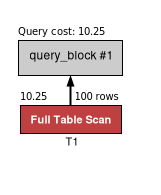
\includegraphics[width=4cm]{images/1-1.png}
\caption{Indexelés nélküli lekérdezés}
\label{fig:schema}
\end{figure}

A grafikus Execution Plan az előbbi ábrával állt elő. Láthatjuk, hogy a T1 -es tábla összes sorát átvizsgálta, a c3 megfelelő értékeinek megkereséséhez. Ez egy nagy táblában egy rendkívül költséges művelet lenne. 
Erre nyújt megoldást az indexelés használata.
\begin{python} 
ALTER TABLE  thesis.T1  ADD INDEX (c3);
\end{python}

\begin{figure}[h!]
\centering
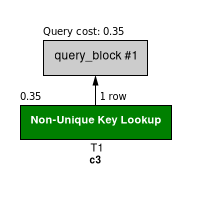
\includegraphics[width=4cm]{images/1-2.png}
\caption{Indexelés nélküli lekérdezés}
\label{fig:schema}
\end{figure}

Újra lefuttatva az előző lekérdezést láthatjuk, hogy a költsége a töredékére csökkent, melynek az az oka, hogy nem kell minden cella értékét megvizsgálni.

Parancs az indexek eltávolításához:
\begin{python} 
ALTER TABLE  thesis.T1  ADD INDEX (c3);
\end{python}

Vizsgáljuk egy kicsit összetettebb lekérdezést: 
\begin{python} 
SELECT MAX(c4), c3, c2 from thesis.T1 WHERE T1.c3=18  group by c2;
\end{python}

\begin{figure}[h!]
\centering
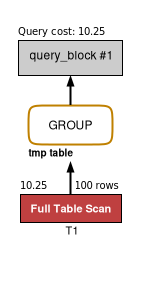
\includegraphics[width=4cm]{images/2-1.png}
\caption{Indexelés nélküli lekérdezés 2.}
\label{fig:schema}
\end{figure}

A lekérdezés elemzésénél két problémát fedezhetünk fel. Az egyik a teljes tábla átvizsgálása csak úgy mint az előző esetben. A másik egy ideiglenes tábla létrejötte ami a lekérdezés idejére memóriát foglal.

\begin{figure}[h!]
\centering
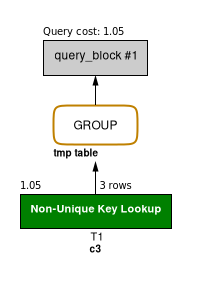
\includegraphics[width=3.5cm]{images/2-2.png}
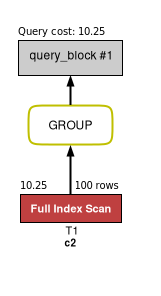
\includegraphics[width=3.5cm]{images/2-3.png}
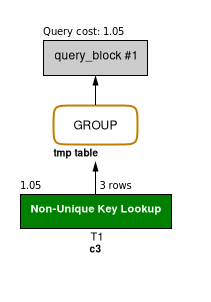
\includegraphics[width=3.5cm]{images/2-4.png}
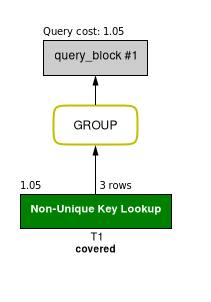
\includegraphics[width=3.5cm]{images/2-5.png}
\caption{Indexelések változatai.}
\label{fig:schema}
\end{figure}


Nézzük a következő négy indexelést.
\begin{itemize} 
\item Első kép: A c3 -as oszlopot indexel láttam el, így az keresés költsége lecsökkent, de az ideiglenes tábla megmaradt.
\item Második kép: A c2 -es oszlopot indexeltem, így az érték keresés a c3 -as oszlopon teljes, de nem jön létre ideiglenes tábla.
\item Harmadik kép: Egyezik az első képpel, pedig a c3 és c2 -es oszlop is indexelve van.
\item Negyedik kép: Közös indexet hoztam létre a c2 és c3 -s oszlopokból így a kétféle indexelés előnyei egyszerre tudnak érvényesülni a lekérdezés során.
\end{itemize} 
Kevert index létrehozása és törlése:
\begin{python}
ALTER TABLE T1 ADD INDEX covered (c3,c2);
ALTER TABLE thesis.T1 DROP INDEX covered;
\end{python}




